Although we will mostly be working in Temperley-Lieb (TL) algebras, we will introduce the notion of a \emph{planar algebra} in this chapter. One of the reasons for this is that the collection of TL algebras can be equipped with a planar structure, yielding the Temperley-Lieb planar algebra, and that trivalent categories have a deep connection to planar algebras as well. The other reason is that our main definitions and some theorems work in planar algebras in general, that is, independent of the nature of the things we `put into the boxes'.

Planar algebras were first defined by Jones in \cite{jones1999planar1}, to help in the study of subfactors. They are designed to graphically capture multilinearity so that one may do calculations using pictures, not unlike the diagrammatic language of (rigid) monoidal categories --- i.e.\ string diagrams, made into a rigorously defined concept by Joyal and Street \cite{joyal1991geometry} --- or other pictorial computation aids, such as found in the theory of tensor networks.

After this chapter we will work out examples almost exclusively in the Temperley-Lieb algebras. This is because the TL \emph{planar} algebra is initial in the category of subfactor planar algebras \cite{peters2010planar}. Then the TL planar algebra can be `lifted' nicely to other subfactor PAs, so the properties and examples we give can, in a sense, be `embedded'.

\subsection{Planar Tangles}
In this section we introduce the basic notion of a \emph{planar tangle}, and give a few examples. We will then describe the operadic nature of these objects. The definition of planar tangle given here is a bit \emph{intuitionistic}. The reader desiring a more mathematical discussion is referred to \textsf{Appendix \ref{app:PA rigor}}, but be aware --- the tangles discussed there are slightly different.

Our first description of \emph{shaded} planar tangles will be in terms of disks, which will eventually turn into rectangles, only to once again become circles when we talk very briefly about \emph{unshaded} planar tangles. We advise the reader to look at \figref{fig:Tangle Examples1}, and to maybe draw their own pictures.

\begin{definition}[Shaded Planar Tangle]\index{Planar Tangle!shaded}\label{def:shaded planar tangle}
Define the set \[\mathfrak{Col} \equiv \mathbb{N}_0\times \{+,-\}\] of \emph{colors}, and pick an element $(n_0,\epsilon_0)\in\mathfrak{Col}$. A \emph{shaded $(n_0, \epsilon_0)$-tangle} $T$ or \emph{shaded tangle} $T$ \emph{with color $(n_0, \epsilon_0)$} is then a disk $D_0$ together with the following extra data.
\begin{itemize}
\item[\textsf{(1)}] In the interior there is a (possibly empty) collection $\mathcal{D}_T$ of disjoint disks $D_i$, $1\leq i \leq \lvert \mathcal{D}_T \rvert$, each with \emph{color} $(n_i, \epsilon_i)$.
\item[\textsf{(2)}] There are $2n_i$ distinct points on the boundary of each disk. Also, for each disk, one of these points is marked with a $\markedPoint$ and called the \emph{first} or \emph{marked point}.
\item[\textsf{(3)}] All distinct points are the endpoints of smooth non-intersecting curves in the interior of $D_0$, and there may also be closed curves not attached to the boundary of any disk. The strings have to be \emph{compatible} with the marked points of all disks in the following sense. Label the marked point of the disk $D_i$ with $\epsilon_i$, then label all other distinct points in a clockwise fashion alternating between $+$ and $-$. A string with one endpoint on an \emph{internal} disk and the other on the \emph{external} disk $D_0$ has to be attached at distinct points with the same sign. For the other two combinations, the signs have to differ.

The curves are called \emph{strings}, their complement in $D_0^\circ - \mathcal{D}_T$ is the set of \emph{regions}. 
\item[\textsf{(4)}] We then put a \emph{shading} on the regions like so: The region on the right of the marked point of the external disk is 
\begin{align*}
	\begin{cases}
		\text{shaded} & \text{if } \epsilon_0 = +\\
		\text{not shaded} & \text{if } \epsilon_0= -
	\end{cases}
\end{align*}
All other regions are then either shaded or not shaded such that no two adjacent regions have the same shading, i.e.\ we have a checkerboard shading. This works because of the compatibility condition in point \textsf{(3)}.

\end{itemize}

Finally, these objects are defined up to isotopy; that is, if you can continuously deform one tangle into another one then both are considered the same.
\end{definition}

Two enlightening examples can be found in \figref{fig:Tangle Examples1}.
\begin{figure}[!htp]
	\centering
	\begin{subfigure}{.49\textwidth}
		\centering
		\begin{tikzpicture}[scale=1.2]
			\coordinate (centerO) at (0,0);
			\coordinate (centerA) at (-0.8,0.6);
			\coordinate (centerB) at (1,0.2);
			\coordinate (centerC) at (0.1,-0.9);
			\coordinate (centerD) at (0.2,1.3);
			\def\radiusO{2cm};
			\def\radiusA{0.5cm};
			\def\radiusB{0.4cm};
			\def\radiusC{0.4cm};
			\def\radiusD{0.3cm};
			\def\helligkeit{30};
			
			% shading
			\begin{scope}
				\path[clip] ($(centerO) + (100:\radiusO)$) -- ($ (centerA) +(90:\radiusA) $) --
					($ (centerA) +(90:\radiusA) $) arc [start angle=90 , end angle=20 , radius=\radiusA] --
					($(centerA) + (20:\radiusA)$) .. controls (0,0.9).. ($ (centerB) +(120:\radiusB) $) --
					($ (centerB) +(120:\radiusB) $) arc [start angle=120 , end angle=70 , radius=\radiusB] --
					($ (centerB) +(70:\radiusB) $) -- ($(centerO) + (30:\radiusO)$) --
					($(centerO) + (30:\radiusO)$) arc [start angle=30 , end angle=100 , radius=\radiusO];				
				\fill[color = gray!\helligkeit, opacity=0.1]  (centerO) circle [radius=\radiusO];
			\end{scope}
			
			\begin{scope}			
				\path[clip] ($(centerA) + (-40:\radiusA)$) -- 
					($ (centerC) +(90:\radiusC) $) arc [start angle=90 , end angle=300 , radius=\radiusC] --
					($ (centerC) +(300:\radiusC) $) -- 
					($(centerO) + (-80:\radiusO)$) arc[start angle=-80, end angle=-100, radius=\radiusO] --
					($ (centerA) +(270:\radiusA) $) arc[start angle=270, end angle=320, radius=\radiusA];
				\fill[color = gray!\helligkeit, opacity=0.1]  (centerO) circle [radius=\radiusO];
			\end{scope}
					
			\draw (centerO) circle [radius=\radiusO];
			\draw[fill=white] (centerA) circle [radius=\radiusA];
			\draw[fill=white] (centerB) circle [radius=\radiusB];
			\draw[fill=white] (centerC) circle [radius=\radiusC];
			\draw[fill=white] (centerD) circle [radius=\radiusD];
			
			\draw (centerA) node {$D_1$};
			\draw (centerB) node {$D_2$};
			\draw (centerC) node {$D_3$};
			\draw (centerD) node {$D_4$};	
	
			%strings
			\draw %[decoration={markings, mark=at position 0.3 with {\arrowreversed{triangle 45}}}, postaction={decorate}] 
				($(centerO) + (100:\radiusO)$) -- ($ (centerA) +(90:\radiusA) $);
			\draw %[decoration={markings, mark=at position 0.3 with {\arrowreversed{triangle 45}}}, postaction={decorate}] 
				($(centerO) + (260:\radiusO)$) -- ($ (centerA) +(270:\radiusA) $);
			\draw %[decoration={markings, mark=at position 0.625 with {\arrow{triangle 45}}}, postaction={decorate}] 
				($(centerO) + (30:\radiusO)$) -- ($ (centerB) +(70:\radiusB) $);
			\draw %[decoration={markings, mark=at position 0.625 with {\arrow{triangle 45}}}, postaction={decorate}] 
				($(centerO) + (-80:\radiusO)$) -- ($ (centerC) +(300:\radiusC) $);
			
			\draw %[decoration={markings, mark=at position 0.625 with {\arrowreversed{triangle 45}}}, postaction={decorate}] 
				($(centerA) + (20:\radiusA)$) .. controls (0,0.9).. ($ (centerB) +(120:\radiusB) $);
			\draw %[decoration={markings, mark=at position 0.3 with {\arrowreversed{triangle 45}}}, postaction={decorate}] 
				($(centerA) + (-40:\radiusA)$) -- ($ (centerC) +(90:\radiusC) $);
			
			\draw[fill=gray!\helligkeit, opacity=0.1] (-1.32,-0.4) circle [x radius = 0.35cm, y radius = 0.8cm, rotate = 30];
			
			% marked points
			\node (markedPointO) at ($(centerO) + (100:\radiusO) + (-0.1,0.1)$) {$\markedPoint$};
			\node (markedPointA) at ($(centerA) + (90:\radiusA) + (-0.1,0.1)$) {$\markedPoint$};
			\node (markedPointB) at ($(centerB) + (70:\radiusB) + (-0.05,0.12)$) {$\markedPoint$};
			\node (markedPointC) at ($(centerC) + (-60:\radiusC) + (0.15,0)$) {$\markedPoint$};
		\end{tikzpicture}
		\caption[]{}\label{subfig:TangleFirstExample}
	\end{subfigure}	
	\begin{subfigure}{.49\textwidth}
		\centering
		\begin{tikzpicture}[scale=1.2]
			\coordinate (centerO) at (0,0);
			\coordinate (centerA) at (0,0);
			\def\radiusO{2cm};
			\def\radiusA{0.5cm};
			\def\helligkeit{30};
			
			% shading
			\begin{scope}
				\path[clip]
				($ (centerA) +(90:\radiusA) $) arc[start angle=90, end angle=270, radius=\radiusA] --
				($(centerO) + (-90:\radiusO)$) arc[start angle=270, end angle=90, radius=\radiusO];
				\fill[color = gray!\helligkeit, opacity=0.1]  (centerO) circle [radius=\radiusO];
			\end{scope}
			\begin{scope}
				\path[clip] 
					($(centerA) + (60:\radiusA)$) .. controls ($(centerA) + (45:\radiusO)$) and ($(centerA) + (-45:\radiusO)$) .. ($ (centerA) +(-60:\radiusA) $) arc[start angle=300, end angle=60, radius=\radiusA];
				\fill[color = gray!\helligkeit, opacity=0.1]  (centerO) circle [radius=\radiusO];				
			\end{scope}
					
			\draw (centerO) circle [radius=\radiusO];
			\draw[fill=white] (centerA) circle [radius=\radiusA];
			
			\draw (centerA) node {$D_1$};	
	
			%strings
			\draw %[decoration={markings, mark=at position 0.3 with {\arrowreversed{triangle 45}}}, postaction={decorate}] 
				($(centerO) + (90:\radiusO)$) -- ($ (centerA) +(90:\radiusA) $);
			\draw %[decoration={markings, mark=at position 0.3 with {\arrowreversed{triangle 45}}}, postaction={decorate}] 
				($(centerO) + (-90:\radiusO)$) -- ($ (centerA) +(-90:\radiusA) $);		
			\draw %[decoration={markings, mark=at position 0.3 with {\arrowreversed{triangle 45}}}, postaction={decorate}] 
				($(centerA) + (60:\radiusA)$) .. controls ($(centerA) + (45:\radiusO)$) and ($(centerA) + (-45:\radiusO)$) .. ($ (centerA) +(-60:\radiusA) $);		
			
			% marked points
			\node (markedPointO) at ($(centerO) + (90:\radiusO) + (-0.1,0.1)$) {$\markedPoint$};
			\node (markedPointA) at ($(centerA) + (90:\radiusA) + (-0.1,0.1)$) {$\markedPoint$};
		\end{tikzpicture}
		\caption[]{}\label{subfig:CondExp Neg}
	\end{subfigure}
\caption[First examples of planar tangles]{Examples of planar tangles. In (\subref{subfig:TangleFirstExample}) we see a $(4,+)$-tangle whose internal disks have colors $(4,+),(2,-),(2,+),$ and $(0,+)$, respectively. The tangle in (\subref{subfig:CondExp Neg}) is $(2,-)$ with a single internal $(4,-)$ disk.}\label{fig:Tangle Examples1}
\end{figure}

Note that the shading is really only a way of encoding the colors of the disk so that they are easier to recognize. It is not necessary to always draw it. The shading is clear as long as one keeps track of the colors and the marked points of each disk.

\bigno Given an $(n,\epsilon)$-tangle $T$ and an $(\tilde{n},\tilde{\epsilon})$-tangle $S$ such that for some internal disk $D_i$ of $T$ we have $(n_i, \epsilon_i)=(\tilde{n},\tilde{\epsilon})$ we can in a natural way define a new $(n,\epsilon)$-tangle $T\circ_i S$. Namely: plug $S$ into $D_i$ such that the marked and all other distinct points of $S$ and $D_i$ coincide, delete the boundary of $S$, and smooth out the strings. Then 
\begin{align*}
\mathcal{D}_{T\circ_i S} = \left(\mathcal{D}_T- \{D_i\}\right) \cup \mathcal{D}_S,
\end{align*}
and we relabel the internal disks in the obvious way, see \eqref{eq:CompositionInternalDiscs} in the appendix. If there is only one internal disk in which we can insert then we will also drop the index and write $\circ$ instead of $\circ_1$.

We can, for example, $\circ_2$-compose the first tangle in \figref{fig:Tangle Examples1} with the second one and obtain
\begin{center}
\begin{tikzpicture}[scale=1]
	\coordinate (centerO) at (0,0);
	\coordinate (centerA) at (-0.8,0.6);
	\coordinate (centerB) at (1,0.2);
	\coordinate (centerC) at (0.1,-0.9);
	\coordinate (centerD) at (0.2,1.3);
	\def\radiusO{2cm};
	\def\radiusA{0.5cm};
	\def\radiusB{0.4cm};
	\def\radiusC{0.4cm};
	\def\radiusD{0.3cm};
	\def\helligkeit{30};
	
	% shading
	\begin{scope}
		\path[clip] ($(centerO) + (100:\radiusO)$) -- ($ (centerA) +(90:\radiusA) $) --
			($ (centerA) +(90:\radiusA) $) arc [start angle=90 , end angle=20 , radius=\radiusA] --
			($(centerA) + (20:\radiusA)$) .. controls (0,0.9).. ($ (centerB) +(120:\radiusB) $) --
			($ (centerB) +(120:\radiusB) $) arc [start angle=120 , end angle=70 , radius=\radiusB] --
			($ (centerB) +(70:\radiusB) $) -- ($(centerO) + (30:\radiusO)$) --
			($(centerO) + (30:\radiusO)$) arc [start angle=30 , end angle=100 , radius=\radiusO];				
		\fill[color = gray!\helligkeit, opacity=0.1]  (centerO) circle [radius=\radiusO];
	\end{scope}
	
	\begin{scope}
		\path[clip]
			($(centerB) + (240:\radiusB)$) 
			.. controls ($(centerB) + (240:\radiusB) + (240:0.5cm)$) and ($(centerB) + (300:\radiusB)+(300:0.5cm)$) .. 
			($ (centerB) +(300:\radiusB) $) arc[start angle=-60, end angle=-120, radius=\radiusB];
		\fill[color = gray!\helligkeit, opacity=0.1]  (centerO) circle [radius=\radiusO];
	\end{scope}
	
	\begin{scope}			
		\path[clip] ($(centerA) + (-40:\radiusA)$) -- 
			($ (centerC) +(90:\radiusC) $) arc [start angle=90 , end angle=300 , radius=\radiusC] --
			($ (centerC) +(300:\radiusC) $) -- 
			($(centerO) + (-80:\radiusO)$) arc[start angle=-80, end angle=-100, radius=\radiusO] --
			($ (centerA) +(270:\radiusA) $) arc[start angle=270, end angle=320, radius=\radiusA];
		\fill[color = gray!\helligkeit, opacity=0.1]  (centerO) circle [radius=\radiusO];
	\end{scope}
			
	\draw (centerO) circle [radius=\radiusO];
	\draw[fill=white] (centerA) circle [radius=\radiusA];
	\draw[fill=white] (centerB) circle [radius=\radiusB];
	\draw[fill=white] (centerC) circle [radius=\radiusC];
	\draw[fill=white] (centerD) circle [radius=\radiusD];
	
	\draw (centerA) node {$D_1$};
	\draw (centerB) node {$D_2$};
	\draw (centerC) node {$D_3$};
	\draw (centerD) node {$D_4$};	

		%strings
	\draw %[decoration={markings, mark=at position 0.3 with {\arrowreversed{triangle 45}}}, postaction={decorate}] 
		($(centerO) + (100:\radiusO)$) -- ($ (centerA) +(90:\radiusA) $);
	\draw %[decoration={markings, mark=at position 0.3 with {\arrowreversed{triangle 45}}}, postaction={decorate}] 
		($(centerO) + (260:\radiusO)$) -- ($ (centerA) +(270:\radiusA) $);
	\draw %[decoration={markings, mark=at position 0.625 with {\arrow{triangle 45}}}, postaction={decorate}] 
		($(centerO) + (30:\radiusO)$) -- ($ (centerB) +(70:\radiusB) $);
	\draw %[decoration={markings, mark=at position 0.625 with {\arrow{triangle 45}}}, postaction={decorate}] 
		($(centerO) + (-80:\radiusO)$) -- ($ (centerC) +(300:\radiusC) $);
	
	\draw %[decoration={markings, mark=at position 0.625 with {\arrowreversed{triangle 45}}}, postaction={decorate}] 
		($(centerA) + (20:\radiusA)$) .. controls (0,0.9).. ($ (centerB) +(120:\radiusB) $);
	\draw %[decoration={markings, mark=at position 0.3 with {\arrowreversed{triangle 45}}}, postaction={decorate}] 
		($(centerA) + (-40:\radiusA)$) -- ($ (centerC) +(90:\radiusC) $);
	\draw
		($(centerB) + (240:\radiusB)$) .. controls ($(centerB) + (240:\radiusB) + (240:0.5cm)$) and ($(centerB) + (300:\radiusB)+(300:0.5cm)$) .. ($ (centerB) +(300:\radiusB) $);
	
	\draw[fill=gray!\helligkeit, opacity=0.1] (-1.32,-0.4) circle [x radius = 0.35cm, y radius = 0.8cm, rotate = 30];
	
	% marked points
	\node (markedPointO) at ($(centerO) + (100:\radiusO) + (-0.1,0.1)$) {$\markedPoint$};
	\node (markedPointA) at ($(centerA) + (90:\radiusA) + (-0.1,0.1)$) {$\markedPoint$};
	\node (markedPointB) at ($(centerB) + (70:\radiusB) + (-0.05,0.12)$) {$\markedPoint$};
	\node (markedPointC) at ($(centerC) + (-60:\radiusC) + (0.15,0)$) {$\markedPoint$};
\end{tikzpicture}
\end{center}

This operation of inserting planar tangles into like-colored internal discs of another tangle is called \emph{composition}, and with it we have pretty much already defined the \emph{colored planar operad} $\mathfrak{P}$, see e.g.\ \cite[p 561 f]{loday2012algebraic}.\footnote{If you know about operads then you may see the planar operad as a more `pedantic' version of the \emph{little disks} operad} What this really means is that, for all intents and purposes, we have a collection of things --- in this case, all planar tangles --- and on this collection we define a notion of \emph{composition} that is associative and unital, where `unitality of composition'  means that there are some elements $\id_{(n_i,\epsilon_i)}$ in our collection such that $T\circ_i \id_{(n_i,\epsilon_i)} = T$, whenever this composition is possible.

It is immediately clear what these units are in our case: For fixed $(n,\epsilon)$ they are the unique $(n,\epsilon)$-tangle with exactly one internal $(n,\epsilon)$-disc, and strings only connecting the internal and the external disks s.t.\ both marked points are endpoints of the same string. For example, the following is $\id_{(2,-)}$:
\begin{align*}
\id_{(2,-)} =\,
\begin{tikzpicture}[scale=0.8, baseline]
	\coordinate (O) at (0,0);
	\def\radiusO{2cm};
	\def\radiusA{0.5cm};
	\def\helligkeit{30};
%	
	% shading
	\begin{scope}
		\path[clip]
			($ (O) +(120:\radiusO) $) arc[start angle=120, end angle=240, radius=\radiusO] --
			($ (O) +(240:\radiusA) $) arc[start angle=240, end angle=120, radius=\radiusA] ;
		\fill[color = gray!\helligkeit, opacity=0.1]  (O) circle [radius=\radiusO];
	\end{scope}
	\begin{scope}
		\path[clip] 
			($ (O) +(60:\radiusO) $) arc[start angle=60, end angle=-60, radius=\radiusO] --
			($ (O) +(-60:\radiusA) $) arc[start angle=-60, end angle=60, radius=\radiusA] ;
		\fill[color = gray!\helligkeit, opacity=0.1]  (O) circle [radius=\radiusO];				
	\end{scope}
%			
	\draw (O) circle [radius=\radiusO];
	\draw[fill=white] (O) circle [radius=\radiusA];
%
		%strings
	\draw %[decoration={markings, mark=at position 0.3 with {\arrowreversed{triangle 45}}}, postaction={decorate}] 
		($(O) + (120:\radiusO)$) -- ($ (O) + (120:\radiusA) $);
	\draw %[decoration={markings, mark=at position 0.3 with {\arrowreversed{triangle 45}}}, postaction={decorate}] 
		($(O) + (60:\radiusO)$) -- ($ (O) + (60:\radiusA) $);		
	\draw %[decoration={markings, mark=at position 0.3 with {\arrowreversed{triangle 45}}}, postaction={decorate}] 
		($(O) + (-120:\radiusO)$) -- ($ (O) + (-	120:\radiusA) $);
	\draw %[decoration={markings, mark=at position 0.3 with {\arrowreversed{triangle 45}}}, postaction={decorate}] 
		($(O) + (-60:\radiusO)$) -- ($ (O) + (-60:\radiusA) $);		
%	
	% marked points
	\node (markedPointO) at ($(O) + (120:\radiusO) + (-0.1,0.1)$) {$\markedPoint$};
	\node (markedPointA) at ($(O) + (120:\radiusA) + (-0.2,0.1)$) {$\markedPoint$};	
\end{tikzpicture}
\end{align*}
As the symbol already implies it also serves as the identity, since for any $(2,-)$-tangle $T$ we clearly have $\id_{(2,-)} \circ T = T$. 

For $x\in\mathfrak{Col}$ we define $\mathcal{T}_x$ to be the free complex vector space on the set of all planar $x$-tangles. These spaces are often called \emph{$x$-box spaces}\footnotemark, as explained in the following.
Note that $\mathcal{T}_{(n,+)}\cong \mathcal{T}_{(n,-)}$ --- every tangle can be defined with the opposite shading.
\footnotetext{Strictly speaking this name only makes sense for shaded tangles}

\bigno
We promised that there is also a description of tangles in terms of rectangles (or \emph{boxes}) instead of discs. This is sometimes easier, and it surely is easier to draw. To obtain it, simply replace all disks by rectangles (or blow up the disks into rectangles, if you will) so that half of the distinct points is along the top edge and the other half is along the bottom edge, and so that on left of the marked point is a corner of the rectangle.

Then we further impose that in this description the marked point be the left-most point on the top. This can always be done by choosing an appropriate representative of the isotopy class, and it is commonly referred to as the \emph{standard form} of the tangle. It allows us to draw pictures even simpler: The symbol $\markedPoint$ doesn't need to be put next to the marked points anymore, as we now know exactly where they are.

\bigno
In terms of boxes it is now easier to talk about an involution that exists on planar tangles. This involution ${}^*$ yields the \emph{adjoint} $T^*$ of a tangle $T$ as follows.
\begin{itemize}
\item[\textsf{$\bullet$}] Take the tangle in standard form.
\item[$\bullet$] Flip it horizontally, i.e.\ along the horizontal axis.
\item[$\bullet$] Interpret the result as a tangle in standard form --- that is, the point that was the ``last'' point (when enumerating in a clockwise) before the flip is now the marked point.
\item[$\bullet$] Note that this operation reversed the shading. But we want the adjoint to have the same color, so invert the shading.
\end{itemize}
That this is indeed involutive, i.e.\ ${}^{**}=\id$, is an easy exercise.

\bigno
Before we go on, let us list some planar tangles that we will encounter a few times.
\subsection*{A Few Important Tangles}\addcontentsline{toc}{subsection}{A Few Important Tangles}
There are a few tangles that deserve to be mentioned explicitly. All of these tangles can be defined for any box space, so we will only give a few easy examples. Arguably the most important one, the \emph{multiplication tangle}, is given by stacking tangles on top of each other, na\"ively speaking. Its pictorial representation can be found after the definition of planar algebras.

The (second) most important one, which will be used all the time in this thesis, is the \emph{rotation tangle} or \emph{one-click rotation} $\mathsf{rot}:\mathcal{T}_{(n,\pm)}\rightarrow \mathcal{T}_{(n,\mp)}$. An example can be found in \figref{fig:rotation tangle}. Note that what makes it a `rotation' is that the marked point of the internal box is offset by one w.r.t.\ the marked point of the exterior box.

\begin{figure}[!htp]\centering
	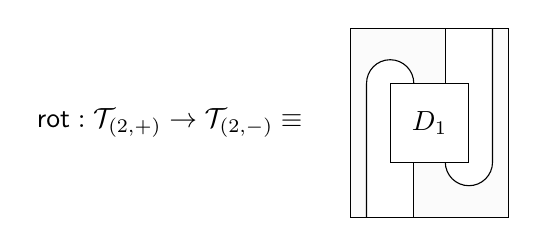
\begin{tikzpicture}
		\node (text) at (-3.3,0) {$\mathsf{rot}:\mathcal{T}_{(2,+)}\rightarrow\mathcal{T}_{(2,-)} \equiv$};
		\def\helligkeit{30};
		\begin{scope}
			\path[clip]
				(-0.2,0.5) arc[start angle=0, end angle=180, radius=3mm] -- ++(0,-1.7) -- ++(-0.2,0) -- ++(0,2.4) -- ++(1.2,0) -- ++(0,-0.7);
			\fill[color = gray!\helligkeit, opacity=0.1]  (-1,-1.2) rectangle (1,1.2);
		\end{scope}
		\begin{scope}
			\path[clip]
				(0.2,-0.5) arc[start angle=180, end angle=360, radius=3mm] -- ++(0, 1.7) -- ++(0.2,0) -- ++(0,-2.4) -- ++(-1.2,0) -- ++(0,0.7);
			\fill[color = gray!\helligkeit, opacity=0.1]  (-1,-1.2) rectangle (1,1.2);
		\end{scope}
		
		\draw[fill= white] (-0.5,-0.5) rectangle (0.5,0.5);
		\node (O) at (0,0) {$D_1$};
		\draw (-1,-1.2) rectangle (1,1.2);
		\draw (-0.2,0.5) arc[start angle=0, end angle=180, radius=3mm] -- ++(0,-1.7);
		\draw (0.2,-0.5) arc[start angle=180, end angle=360, radius=3mm] -- ++(0,1.7);
		\draw (0.2, 0.5) -- ++(0,0.7);
		\draw (-0.2, -0.5) -- ++(0,-0.7);
	\end{tikzpicture}
	\caption[The rotation tangle]{The shaded rotation tangle for $(2,+)$-tangles. All boxes are in standard form. The shading is supplied for clarity.}
	\label{fig:rotation tangle}
\end{figure}

\bigno Now the notation will be getting a bit messy, but we promise that the reader only has to endure this for a short while. We can also define the \emph{inclusion tangle} $\textsf{inc}_{k,\pm}^{k+1}$ (see \figref{fig:InclusionTangle}), which takes a $(k,\pm)$-tangle $S$ and maps it to the $(k+1,\pm)$-tangle $\textsf{inc}_{k,\pm}^{k+1}\circ_1 S$. It of course also makes sense to then define the general symbol $\textsf{inc}_{k,\pm}^{l}\equiv \textsf{inc}_{l-1,\pm}^{l}\circ \ldots \circ \textsf{inc}_{k,\pm}^{k+1}$ for $l>k$, this is just `including the inclusion'.

There also exists a sort of `converse' for the inclusion, commonly called the \emph{conditional expectations tangle} $\mathcal{E}_{k+1,\pm}^{k}$ as seen in \figref{fig:ConditionalExpectationTangle}, taking $(k+1,\pm)$-tangles to $k$-tangles with the same shading for the marked point. For this tangle an obvious generalization $\mathcal{E}_{k+1,\pm}^{l}$, for $l\leq k$, is readily defined.

\begin{figure}[!htp]\centering
	\begin{subfigure}{0.5\textwidth}\centering
		\begin{tikzpicture}[scale=0.8, every node/.style={scale=0.8}]
			\coordinate (centerO) at (0,0);
			\def\radiusO {2cm};
			\def\radiusA {.7cm};
		
			\begin{scope}		
				\path[clip] ($(centerO)+(90:\radiusO)$) -- 
					($(centerO)+(90:\radiusA)$)  arc [start angle=90, end angle=-90, radius=\radiusA] --
					($(centerO) + (-90:\radiusO)$) --
					($(centerO)+(-90:\radiusO)$) arc [start angle=270, end angle=315, radius=\radiusO] --
					($(centerO)+(-45:\radiusO)$) -- 
					($(centerO) + (45:\radiusO)$) arc [start angle=45, end angle=90, radius=\radiusO];	
				\fill[color = gray!30, opacity=0.1]  (centerO) circle [radius=\radiusO];
			\end{scope}
			
			\draw (centerO) circle [radius=\radiusO];
			\draw (centerO) circle [radius=\radiusA];
			\draw ($(centerO)+(90:\radiusO)$) -- ($(centerO)+(90:\radiusA)$);
			\draw ($(centerO)+(-90:\radiusO)$) -- ($(centerO)+(-90:\radiusA)$);
			\draw ($(centerO)+(45:\radiusO)$) -- ($(centerO) + (-45:\radiusO)$);
			\draw (centerO) node {$D_1$};
			
			\draw ($(centerO)+(90:\radiusO) + (-0.1,0.1)$) node {$\markedPoint$};
			\draw ($(centerO)+(90:\radiusA) + (-0.1,0.1)$) node {$\markedPoint$};
		\end{tikzpicture}
		\caption[]{}
		\label{fig:InclusionTangle}
	\end{subfigure}
	\begin{subfigure}{0.49\textwidth}\centering
		\begin{tikzpicture}[scale=0.8, every node/.style={scale=0.8}]
			\coordinate (centerO) at (0,0);
			\def\radiusO {2cm};
			\def\radiusA {.7cm};		
		
			\begin{scope}		
				\path[clip] ($(centerO)+(90:\radiusO)$) -- 
					($(centerO)+(90:\radiusA)$)  arc [start angle=90, end angle=45, radius=\radiusA] --
					($(centerO)+(45:\radiusA)$) .. 
						controls ($(centerO)+(40:1.6cm)$) and ($(centerO)+(0:1.2cm)$) ..
						($(centerO)+(0:1.2cm)$)..
						controls ($(centerO)+(0:1.2cm)$) and ($(centerO)+(-40:1.6cm)$) ..
						($(centerO)+(-45:\radiusA)$) --
					($(centerO)+(-45:\radiusA)$) arc [start angle=-45, end angle=-90, radius=\radiusA] --
					($(centerO)+(-90:\radiusO)$) arc [start angle=-90, end angle=90, radius=\radiusO];	
				\fill[color = gray!30, opacity=0.1]  (centerO) circle [radius=\radiusO];
			\end{scope}
			
			\draw (centerO) circle [radius=\radiusO];
			\draw (centerO) circle [radius=\radiusA];
			\draw ($(centerO)+(90:\radiusO)$) -- ($(centerO)+(90:\radiusA)$);
			\draw ($(centerO)+(-90:\radiusO)$) -- ($(centerO)+(-90:\radiusA)$);
			\draw ($(centerO)+(45:\radiusA)$) .. 
				controls ($(centerO)+(40:1.6cm)$) and ($(centerO)+(0:1.2cm)$) ..
				($(centerO)+(0:1.2cm)$)..
				controls ($(centerO)+(0:1.2cm)$) and ($(centerO)+(-40:1.6cm)$) ..
				($(centerO)+(-45:\radiusA)$);

			\draw (centerO) node {$D_1$};
			
			\draw ($(centerO)+(90:\radiusO) + (-0.1,0.1)$) node {$\markedPoint$};
			\draw ($(centerO)+(90:\radiusA) + (-0.1,0.1)$) node {$\markedPoint$};
		\end{tikzpicture}
		\caption[]{}
		\label{fig:ConditionalExpectationTangle}
	\end{subfigure}
	
	\caption[Inclusion and conditional expectation tangles]{(\subref{fig:InclusionTangle}) The inclusion tangle $\textsf{inc}_{1,+}^{2}:\mathcal{T}_{(1,+)}\rightarrow\mathcal{T}_{(2,+)}$ and
		(\subref{fig:ConditionalExpectationTangle})	the conditional expectation tangle $\mathcal{E}_{2,+}^{1}$.
	}
\end{figure}

Finally, we can also define another conditional expectation tangle that closes to the left. But observe that this one will switch the shading. We then get two a priori distinct notions of what we call  \emph{trace}, by fixing one of ways of building conditional expectation tangles (i.e.\ closing left or right), and successively applying it until the result lives in either $\mathcal{T}_{(0,+)}$ or $\mathcal{T}_{(0,-)}$.

\bigno\bigno

Before going on to defining planar algebras, let us lose a few words on \emph{unshaded tangles}. The name already suggests the main difference: they do not come with a shading. This means that the set of colors is then really just the set of natural numbers, i.e.\ $\mathfrak{Col} =\mathbb{N}_0$, and we consequently require an unshaded $n$-tangle to have $n$ distinct points on the boundary --- in the shaded case we needed an even number of points so that shading is actually possible. It is clear that then, in general, a representation in terms of boxes is not possible --- only when the number of points is even. 
\subsection{Planar Algebras}
Here, again, we will discuss \emph{shaded planar algebras} first, after which we briefly mention the unshaded case. In the fewest possible words,
\begin{center}
\begin{minipage}{0.8\textwidth}
A shaded planar algebra is an operad homomorphism from $\mathfrak{P}$ to a colored operad $\mathfrak{V}$ of vector spaces.\footnotemark
\end{minipage}
\end{center}
\footnotetext{almost verbatim \cite[Def.\ 2.2]{jones2000planarBipartite}}
That sounds weird, so let us make it more precise. Consider a collection $P\equiv\left\{ P_x \right\}_{x\in\mathfrak{C}}$ of vector spaces, indexed by a set of colors. This collection lives in the symmetric monoidal category $\catname{Vect}_k$ of vector spaces over some field $k$, and we can look at things like
\begin{align*}
\mathrm{Hom}\left( \bigotimes_{x\in U} P_x, P_y\right),\quad \text{for } U\subset\mathfrak{Col},
\end{align*}
i.e.\ linear maps from the tensor product of some of the vector spaces to another vector space in $P$. To discover the operadic structure $\mathfrak{V}$ coming with $P$, we make use of the so-called \emph{tensor-hom adjunction}, which tells us that there is an isomorphism
\begin{align*}
\mathrm{Hom}\left( A\tensor B, C \right)\cong \mathrm{Hom}\left( A,\mathrm{Hom}\left( B,C \right) \right),
\end{align*}
natural in $A, C$ for every $B$ \cite[p 505 f]{aluffi2009algebra} --- basically currying.\footnote{Indeed, the isomorphism may be viewed as
\begin{align*}
A\tensor B \rightarrow C \overset{\sim}{\longleftrightarrow} A\rightarrow\left( B\rightarrow C \right)
\end{align*}
}
Let $U,V\subset \mathfrak{Col}$ be finite, and $x,y\in\mathfrak{Col}$. For any two maps
\begin{align*}
\bigotimes_{a_i\in U} P_{a_i}\morphism{f} P_x \qquad\text{and}\qquad \bigotimes_{b_j\in V} P_{b_j}\morphism{g} P_y,
\end{align*}
there exists a natural composition whenever $x=b_j$. To see this, fix some $l$ s.t.\ $x=b_l$.
By the tensor-hom adjunction there exists a unique map
\begin{align*}
P_x = P_{b_l}  \overset{\tilde{g}}{\dashrightarrow} \mathrm{Hom}\left( \bigotimes_{b\in V-\{b_l\}} P_b, P_y \right)
\end{align*}
corresponding uniquely to $g$. Then we define the composition $g\diamond_l f$ to be the map corresponding to
\begin{align*}
\tilde{g} \circ f \in& \,\mathrm{Hom}\left( \bigotimes_{a_i\in U} P_{a_i}, \mathrm{Hom}\left( \bigotimes_{b\in V-\{b_l\}} P_b, P_y  \right) \right)\\[2em]
\cong& \, \mathrm{Hom}\left(  \bigotimes_{a \in U\cup V-\{b_l\}} P_{a}, P_y\right)
\end{align*}
via the tensor-hom adjunction.
It is now easy to think about what would be considered an `operad homomorphism', and we record this in the following definition.
\begin{definition}[Planar Algebra]\index{Planar Algbra}\label{def:Planar Algebra}
The collection $P$ becomes a planar algebra by choosing an interpretation $Z:\mathfrak{P}\rightarrow\mathfrak{V}$ of planar tangles in terms of linear maps, compatible with the operadic structures.

That is, an $(n,\epsilon)$-tangle $T$ with $k$ internal disks will be mapped to the linear transformation
\begin{align*}
Z(T): \bigotimes_{i=1}^k P_{(n_i,\epsilon_i)} \rightarrow P_{(n,\epsilon)},
\end{align*}
i.e.\ a linear map from the spaces associated with the inner boundaries of the tangle to space associated with the outer boundary. If $k=0$ then the empty tensor product is the underlying field, and $Z(T)$ is therefore a vector in $P_{(n,\epsilon)}$. We also impose $Z(\id_{(n,\epsilon)}) = \id_{(n,\epsilon)}$.

The compatibility is then that $Z$ is something akin to a homomorphism, i.e.\
\begin{align*}
Z(T\circ_i S) = Z(T)\diamond_i Z(S)
\end{align*}
We will also call $P$ itself a planar algebra, and use $Z$ to denote the homomorphism in general.
\end{definition}

We have already implicitly encountered one example. If $P_x = \mathcal{T}_x$ for $x\in\mathfrak{Col}$, then we get an obvious planar algebra structure --- the trivial one --- and can easily see that each $\mathcal{T}_{(n,\epsilon)}$ is turned into an associative algebra with multiplication
\begin{align*}\mathrm{mult}_n \equiv \,
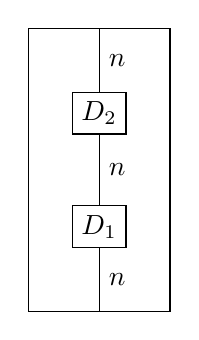
\begin{tikzpicture}[scale=0.9, baseline]
	\coordinate (O) at (0,0);
	\node[draw] (A) at (0,0.8) {$D_2$}; 
	\node[draw] (B) at (0,-0.8) {$D_1$};
	\def\radiusO{2cm};
	\def\radiusA{.6cm};
%
	\draw (-1,-2) rectangle (1,2);
	\draw (0,2) -- node[right] {$n$} (A.north);
	\draw (A.south) -- node[right] {$n$} (B.north);
	\draw (B.south) -- node[right] {$n$} (0,-2);
\end{tikzpicture}\,.
\end{align*}
Here and in the following, an $n$ next to a string implies that there are actually $n$ parallel copies of that string, and the marked points are at the top left of the respective box, as discussed previously. The shading was not drawn, because it is implicitly clear.

The associativity of the multiplication is easily seen by simply remembering  that tangles are defined up to isotopy so that 
\[ \mult_n \circ_1 \mult_n \sim \mult_n\circ_2 \mult_n. \]
Note that this is even commutative if $n=0.$

\subsection*{Additional Stuff, Structure, Property}\addcontentsline{toc}{subsection}{Additional Stuff, Structure, Property}
So far the family of planar $(n,\epsilon)$-tangles is quite large, because there can be an arbitrary collection of closed curves on the inside. Usually, the planar algebras one encounters have an additional property regarding these.

\begin{definition}[Modulus]\index{Modulus!Planar Algebra}
Let $P$ be a planar algebra over $\mathbb{F}$. Let $T$ be a tangle with a closed curve, and let $\hat{T}$ be the same tangle without that curve.

If there exists a
\begin{align*}
\delta \equiv 
\begin{cases}
	\delta_+ &\text{if region bounded by curve is shaded} \\
	\delta_- &\text{if region bounded by curve is unshaded}	
\end{cases}
\in\mathbb{F}
\end{align*}
such that
\begin{align*}
Z(T) = \delta Z(\hat{T})
\end{align*}
then $P$ is said to have \emph{shaded (unshaded) modulus} $\delta_+$ ($\delta_-$). We will only ever encounter the case where $\delta_+ = \delta_->0$, and we then simply say that \emph{$P$ has (positive) modulus $\delta$.}
\end{definition}
\noindent Looking back at the Temperley-Lieb algebras, $\delta$ is also called \emph{loop value}.

\bigno
We may also want to carry the involution on tangles to planar algebras.
\begin{definition}[Planar ${}^*$-algebra]
A planar algebra $P$ over $\mathbb{F}$ is called a \emph{planar ${}^*$-algebra} if $\mathbb{F}$ has a conjugation and if for all colors $x\in\mathfrak{Col}$ the vector space $P_x$ possesses an antilinear involution, such that this involution commutes with the one on planar tangles, that is
\begin{align*}
Z_T(v_1, \ldots, v_k)^* = Z_{T^*}(v_1^*,\ldots, v_k^*)
\end{align*}
for an $n$-tangle $T$ with $k$ internal boxes.
\end{definition}
If the vector spaces are even $C^*$-algebras with that involution, then one speaks of a \emph{planar $C^*$-algebra}.  We only encounter planar algebras consisting of complex vector spaces in this thesis.

The motivation for planar algebras came from the study of subfactors. As famously proven by Jones in \cite[Chapter 4]{jones1999planar1} subfactors give rise to a certain type of planar algebra, and every planar algebra of that type comes from a subfactor. We will now define these important PAs. 
\begin{definition}[Subfactor Planar Algebra]\index{Planar Algebra!Subfactor}
A planar ${}^*$-algebra $S$ is a \emph{subfactor planar algebra} if
\begin{itemize}
\item[\textsf{(i)}] All vector spaces are finite-dimensional, and $\dim S_{0,\pm}=1$. This last property is sometimes called \emph{connectedness}.
\item[\textsf{(ii)}] It is \emph{spherical}: The assignment of complex numbers to labelled\footnotemark\footnotetext{If $T$ is a $(0, \epsilon_0)$-tangle with internal disks $D_i$, then a \emph{labelling} is an element in the range of $Z_T$, drawn as $T$ with some vectors $v_i\in S_{(k_i, \epsilon_i)}$ in the preimage `inserted' into its $i$th internal disk. A labelling is thus equivalently a choice of elements in the domain of $Z_T$.}
 $(0,\pm)$-tangles is invariant under isotopies of the 2-sphere, cf.\ \textsf{Appendix \ref{Appendix:Categories}}. This assignment is called \emph{partition function}. Sphericality means that left and right traces coincide.
\item[\textsf{(iii)}]We can define a positive-definite bilinear form $\langle v,w \rangle\equiv \mathrm{tr}(w^* v)$, which is then called the \emph{inner product}.
\end{itemize}
\end{definition}

A subfactor planar algebra thus has single modulus, as implied by items \textsf{(i)} and \textsf{(ii)}.

\subsection{The Temperley-Lieb Planar Algebra}
The Temperley-Lieb planar algebra $\mathfrak{TL}$ is as simple as it gets, and we can define it as a shaded PA with modulus. All Temperley-Lieb diagrams are already in standard form when interpreted as planar tangles with no internal boxes. It is then clear how to put the two different shadings on a tangle, by simply choosing the color of the first region after the marked point. That way we already get all vector spaces $TL_{(n,\epsilon)}$ whose colors are in $\mathbb{N}\times\{+,-\}$. The two remaining vector spaces $TL_{0,\pm}$ are identified with $\mathbb{C}$.

Tangles with internal boxes act on this collection of vector spaces in an obvious way: TL basis diagrams are tangles, so we just compose and extend by linearity, for each internal disk. Thus by labelling a planar tangle with vectors in TL algebras we get a (multi-)linear map between (products of) these algebras.

Looking back at the definition of subfactor planar algebra, we see that the TL PA almost satisfies it. It has a natural ${}^*$-structure, and the first two items in the definition follow immediately. The inner product, however, need not exist: the bilinear form defined by the trace is not necessarily positive definite, depending on the loop value. Taking quotients by the elements $x$ for which $\langle x,x \rangle=0$ then yields vectors spaces with honest inner products. We can thus turn every Temperley-Lieb planar algebra into a subfactor PA.

We paraphrase \cite{peters2010planar} almost verbatim:
\begin{fact}If $S$ is any subfactor planar algebra with modulus $\delta$, then the obvious `embedding' of the TL PA, i.e.\ the planar algebra homomorphism
\begin{align*}
\mathfrak{TL}\hookrightarrow S,
\end{align*}
given by interpreting Temperley-Lieb tangles as tangles without input disks, is injective if $\delta \geq 2$, otherwise its kernel is the radical of the bilinear form, so that modding out the kernel gives an injective planar algebra homomorphism.
\end{fact}
When we define \emph{perfect tangles} $T$ in the next chapter it will become clear that these are not in the kernel of that map: They are defined such that $\langle T,T \rangle \propto \mathrm{tr}(\mathbf{1_k})$, where $\mathbf{1}_k$ is the tangle that is the multiplicative unit for the multiplication of $k$-tangles.

%\subsection{Instructive Example: The Planar Algebra of a Bipartite Graph}
%Here we will show how, given a bipartite graph, one may construct an associated planar algebra. If one chooses to make this algebra into a planar $*$-algebra, then one obtains a $C^*$-algebra, and we will show how to obtain its Bratelli diagram. \ruggedtodo[inline]{somehow write:} [easy since finite-dimensional $\leadsto$ matrix algebras]


\section{Trivalent Categories}
Trivalent categories, as defined in \cite{Morrison2017Trivalent}, have the nice property that the calculations within are basically calculations in a certain unshaded planar algebra with additional constraints.

We will first write down their category-theoretic definition, but from then on only use string diagrams to apply the methods from the theory of planar algebras. In the vein of the seminal paper we first introduce a few preliminary notions.

The first one is \emph{evaluability}: a monoidal $\mathbb{F}$-linear category is \emph{evaluable} if and only if $\dim\mathrm{Hom}(1,1) = 1$, and that endomorphism space is identified with $\mathbb{F}$ by sending the empty string diagram to $1\in \mathbb{F}$.

Secondly, to rule out a certain degeneracy like before, we call a pivotal category \emph{non-degenerate} iff for every nonzero morphism $f:X\rightarrow Y$ we can find a morphism $f^\prime:Y\rightarrow X$ such that the trace $\mathrm{tr}\left( f^\prime\circ f \right)\in\mathrm{Hom}(1,1)$ is not zero.

For a fixed object $X$ we introduce the notation 
\begin{align*}
\mathcal{C}_n \equiv\mathrm{Hom}\left( 1, X^{\tensor n} \right).
\end{align*}
These vector spaces form an unshaded planar algebra, so far only formally. After the next definition we will understand that $\mathcal{C}_n$ is the span of open planar trivalent graphs with $n$ boundary points, up to isotopy rel boundary, so that only tangles with internal disks of color at most $3$ play any role at all.

\begin{definition}[Trivalent Category]
A triple $\left( \mathcal{C},X,\tau \right)$ forms a \emph{trivalent category} if
\begin{itemize}
\item[•] $\mathcal{C}$ is a strict pivotal $\mathbb{C}$-linear category that is evaluable and non-degenerate
\item[•] $X$ is a self-dual simple object such that 
	\begin{align*}
		\dim\mathcal{C}_1 = 0,\qquad \dim\mathcal{C}_2 = 1,\qquad \dim\mathcal{C}_3 = 1
    \end{align*}
\item[•] $\tau \in \mathcal{C}_3$, called the \emph{trivalent vertex}, is rotationally invariant, that is 
	\begin{align*}
		\begin{tikzpicture}[scale=0.5, baseline]
			\node[draw] (t) at (0,0) {$\tau$};
			\foreach \x in {-0.3,0} \draw ($(t.north) + (\x,0)$) .. controls +(\x,0.5) .. ++(\x,1);
		% 
			\draw ($(t.north) + (0.3,0)$) arc[start angle=180, end angle=0, radius=5mm] --
				++ (0,-1) arc[start angle=0, end angle=-180, radius=1.3cm] -- ++ (0,2);
		\end{tikzpicture}
		\, = \,
			\begin{tikzpicture}[scale=0.5, baseline]
			\node[draw] (t) at (0,0) {$\tau$};
			\foreach \x in {-0.3,0,0.3} \draw ($(t.north) + (\x,0)$) .. controls +(\x,0.5) .. ++(\x,1);
		\end{tikzpicture}\,,
	\end{align*}
	and $\mathcal{C}$ is generated by $\tau$. This means that every morphism is obtained from tensoring and adding identities, (co)evaluations, the self-duality, and trivalent vertices.
\end{itemize}
\end{definition}
Let from now on $\mathcal{C}$ be as in the definition. The object $X$ is actually symmetrically self-dual, meaning that there exists an isomorphism $\phi:X\morphism{\sim} X^*$ with $\phi^* = \phi$. This follows from the non-degeneracy and the dimension of $\mathcal{C}_3$, see Lemma 2.2 in \cite{Morrison2017Trivalent}.

\bigno It is customary to drop the label of the morphism and to simply denote it by a trivalent vertex. Then every string diagram will be an open planar trivalent graph, where strings correspond to simple objects, and two graphs isotopic rel boundary correspond to the same morphism (the self-duality is not drawn). Our category is \emph{defined} to behave nicely, so we can use planar isotopy to deform graphs. For us it is not necessary to reinterpret the graphs as morphisms, since we are only using the graphical calculus.

\bigno Because of the non-degeneracy and the dimensional restrictions we can already extract a few necessary parameters for trivalent categories. For one, any diagram containing the \emph{lollipop}
\begin{align*}
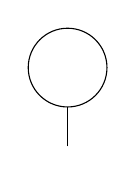
\begin{tikzpicture}[scale=0.5]
	\draw (1,0) arc[start angle=0, end angle=360, radius=1cm];
	\draw (0,-2) -- (0,-1);
\end{tikzpicture}
\end{align*}
as a subgraph is zero, since $\dim\mathcal{C}_1=0$.

Next, a loop (a circle shape) is an element in $\mathbb{C}$, called $d$.  This value must be nonzero, because the loop is the basis element of $\mathcal{C}_2$ composed with its dual.

On the other hand, the following element is in $\mathcal{C}_2$ and must thus be a scalar multiple of the single string,
\begin{align*}
\begin{tikzpicture}[scale=1, baseline]
	\node (A) at (-0.5,-0.8) {};
	\node (B) at (0.5,-0.8) {};
	\foreach \node in {A, B}
		\foreach \x in {-0.3,0,0.3} 
			\draw (\node.north) .. controls +(\x,0.5) .. ++(\x,1);
	\draw ($(A.north) + (0.3,1)$) arc[start angle=180, end angle=0, radius=2mm];
	\draw ($(A.north) + (0,1)$) arc[start angle=180, end angle=0, radius=5mm];
	\draw ($(A.north) + (-0.3,1)$) -- ++(0,0.5);
	\draw ($(B.north) + (0.3,1)$) -- ++(0,0.5);
\end{tikzpicture} \, = \, b\cdot \,
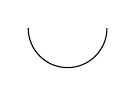
\begin{tikzpicture}[baseline]
	\draw (-0.5,0.3) arc[start angle=180, end angle=360, radius=5mm];
\end{tikzpicture}\,,
\end{align*}
and like before putting a cap on this must yield $bd\neq 0$, so the parameter $b$  must be nonzero. The trivalent vertex can be normalized so that we always take $b=1$.

Finally, we can rotate and compose trivalent vertices such that the result lives again in $\mathcal{C}_3$ (just imagine all legs bent up), and it must thus be some multiple of the trivalent vertex itself, like so:
\begin{align*}
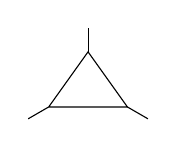
\begin{tikzpicture}[baseline]
	\coordinate (a) at (0,0.5);
	\coordinate (b) at (-0.5,-0.2);
	\coordinate (c) at (0.5,-0.2);
	\draw (a) -- ++ (0,0.3);
	\draw (b) -- ++(210:3mm);
	\draw (c) -- ++(330:3mm);
	\path[draw] (b) -- (a) -- (c) -- (b);
\end{tikzpicture}\, = t\cdot \,
\begin{tikzpicture}[baseline]
	\foreach \angle in {90, 210, 330}
		\draw (0,0) -- ++(\angle:5mm);
\end{tikzpicture}.
\end{align*}
However, coming from the composition, $t$ could actually vanish here.

\bigno In their paper, Morrison \emph{et al} then started classifying trivalent categories by
\begin{itemize}
\item[\text{a)}] the dimensions of the morphism spaces $\mathcal{C}_n$, together with
\item[\text{b)}] the parameters $d$ and $t$, often satisfying some polynomial unique to the category.
\end{itemize}

In this paper, we only look at trivalent categories where $\dim\mathcal{C}_4$ is 4-dimensional, and a basis is provided by the set of all planar trivalent graph with 4 four boundary points and no internal faces. Any trivalent category with this property is called a \emph{cubic category}.

Cubic categories have a nice relation for the square (the trivalent graph with four boundary points, four trivalent vertices, and one internal face), and that makes them particularly nice to work with.

\bigno
It is clear how to interpret open trivalent graphs with $n$-boundary points as unshaded $n$-tangles: We only need to agree on the marked points, and blow up each trivalent vertex to an internal $3$-disk, labelled with $\tau$, and we also simply call that disk $\tau$. \emph{Rotational invariance} then means $\mathrm{rot}\tau = \tau$, so the choice of marked point on $3$-disks doesn't actually matter at all.

A caveat is appropriate here: In planar algebras, we used the symbol ${}^*$ do denote the adjoint or dual of a tangle. That symbol, however, is already reserved in trivalent categories for the category-theoretic dual. Thus for a morphism $f$ in a trivalent category, $f^*$ means ``rotate through $\pi$''. Luckily, it is quickly checked that the notion of horizontally reflecting morphisms is just an instance of what has been called \emph{conjugation} before, for example in \cite{wang2010topological}, where conjugation of morphisms $f,g$ in a pivotal $\mathbb{C}$-linear category was defined as an anti-linear operation $\overline{\phantom{f}}$ that switches source and target of a morphism and satisfies
\begin{align*}
\overline{\overline{f}} = f,\qquad\qquad \overline{f\tensor g} = \overline{f}\tensor\overline{g},\qquad\qquad \overline{f\circ g} = \overline{g}\circ \overline{f}.
\end{align*}
Keeping that in mind, translating the following discussion of \emph{perfect tangles} to trivalent categories is then but a quick change in notation.
